\documentclass[twoside]{book}

% Packages required by doxygen
\usepackage{calc}
\usepackage{doxygen}
\usepackage{graphicx}
\usepackage[utf8]{inputenc}
\usepackage{makeidx}
\usepackage{multicol}
\usepackage{multirow}
\usepackage{textcomp}
\usepackage[table]{xcolor}

% NLS support packages
\usepackage[spanish]{babel}
% Font selection
\usepackage[T1]{fontenc}
\usepackage{mathptmx}
\usepackage[scaled=.90]{helvet}
\usepackage{courier}
\usepackage{amssymb}
\usepackage{sectsty}
\renewcommand{\familydefault}{\sfdefault}
\allsectionsfont{%
  \fontseries{bc}\selectfont%
  \color{darkgray}%
}
\renewcommand{\DoxyLabelFont}{%
  \fontseries{bc}\selectfont%
  \color{darkgray}%
}

% Page & text layout
\usepackage{geometry}
\geometry{%
  a4paper,%
  top=2.5cm,%
  bottom=2.5cm,%
  left=2.5cm,%
  right=2.5cm%
}
\tolerance=750
\hfuzz=15pt
\hbadness=750
\setlength{\emergencystretch}{15pt}
\setlength{\parindent}{0cm}
\setlength{\parskip}{0.2cm}
\makeatletter
\renewcommand{\paragraph}{%
  \@startsection{paragraph}{4}{0ex}{-1.0ex}{1.0ex}{%
    \normalfont\normalsize\bfseries\SS@parafont%
  }%
}
\renewcommand{\subparagraph}{%
  \@startsection{subparagraph}{5}{0ex}{-1.0ex}{1.0ex}{%
    \normalfont\normalsize\bfseries\SS@subparafont%
  }%
}
\makeatother

% Headers & footers
\usepackage{fancyhdr}
\pagestyle{fancyplain}
\fancyhead[LE]{\fancyplain{}{\bfseries\thepage}}
\fancyhead[CE]{\fancyplain{}{}}
\fancyhead[RE]{\fancyplain{}{\bfseries\leftmark}}
\fancyhead[LO]{\fancyplain{}{\bfseries\rightmark}}
\fancyhead[CO]{\fancyplain{}{}}
\fancyhead[RO]{\fancyplain{}{\bfseries\thepage}}
\fancyfoot[LE]{\fancyplain{}{}}
\fancyfoot[CE]{\fancyplain{}{}}
\fancyfoot[RE]{\fancyplain{}{\bfseries\scriptsize Generado el Miércoles, 30 de Agosto de 2017 01\-:01\-:02 para F\-I\-U\-B\-E\-R por Doxygen }}
\fancyfoot[LO]{\fancyplain{}{\bfseries\scriptsize Generado el Miércoles, 30 de Agosto de 2017 01\-:01\-:02 para F\-I\-U\-B\-E\-R por Doxygen }}
\fancyfoot[CO]{\fancyplain{}{}}
\fancyfoot[RO]{\fancyplain{}{}}
\renewcommand{\footrulewidth}{0.4pt}
\renewcommand{\chaptermark}[1]{%
  \markboth{#1}{}%
}
\renewcommand{\sectionmark}[1]{%
  \markright{\thesection\ #1}%
}

% Indices & bibliography
\usepackage{natbib}
\usepackage[titles]{tocloft}
\setcounter{tocdepth}{3}
\setcounter{secnumdepth}{5}
\makeindex

% Hyperlinks (required, but should be loaded last)
\usepackage{ifpdf}
\ifpdf
  \usepackage[pdftex,pagebackref=true]{hyperref}
\else
  \usepackage[ps2pdf,pagebackref=true]{hyperref}
\fi
\hypersetup{%
  colorlinks=true,%
  linkcolor=blue,%
  citecolor=blue,%
  unicode%
}

% Custom commands
\newcommand{\clearemptydoublepage}{%
  \newpage{\pagestyle{empty}\cleardoublepage}%
}


%===== C O N T E N T S =====

\begin{document}

% Titlepage & ToC
\hypersetup{pageanchor=false}
\pagenumbering{roman}
\begin{titlepage}
\vspace*{7cm}
\begin{center}%
{\Large F\-I\-U\-B\-E\-R }\\
\vspace*{1cm}
{\large Generado por Doxygen 1.8.6}\\
\vspace*{0.5cm}
{\small Miércoles, 30 de Agosto de 2017 01:01:02}\\
\end{center}
\end{titlepage}
\clearemptydoublepage
\tableofcontents
\clearemptydoublepage
\pagenumbering{arabic}
\hypersetup{pageanchor=true}

%--- Begin generated contents ---
\chapter{server}
\label{md__r_e_a_d_m_e}
\hypertarget{md__r_e_a_d_m_e}{}
Build status\-: \href{https://travis-ci.org/fiuber/appserver}{\tt !\mbox{[}Build Status\mbox{]}(https\-://travis-\/ci.\-org/fiuber/appserver.\-svg?branch=master)}

\section*{Manual de configuracion e instalacion}

\subsection*{Instalacion}

Para la instalacion del A\-P\-P server de manera local se deberan seguir los siguientes pasos\-:


\begin{DoxyItemize}
\item Realizar un clone del repositorio de la siguiente forma \char`\"{}git clone https\-://github.\-com/fiuber/appserver.\-git\char`\"{} previamente navegando al directorio en el que se quiera clonar el repositorio.
\item Correr el script ./lanzar que se encarga hacer el build de la imagen de docker y correrla exponiendo el puerto 5000.
\item Ya se pueden realizar request al App Server en la direccion localhost\-:5000 con el programa postman o similar.
\end{DoxyItemize}

Si en cambio se desea realizar pruebas al servidor de produccion se pueden enviar requests a la direccion \char`\"{}http\-://fiuberappserver.\-herokuapp.\-com/\char`\"{} donde esta el mismo.

\subsection*{Configuracion}

Se incluye un archivo de configuracion por defecto pero el servidor puede ser configurado a gusto utilizando el archivo \char`\"{}\-\_\-\-\_\-init\-\_\-\-\_\-.\-py\char`\"{} ubicado en el directorio \char`\"{}src/\char`\"{} del App Server en donde se encuentran todos los parametros que se pueden variar del servidor tales como\-:


\begin{DoxyItemize}
\item \char`\"{}app.\-config\mbox{[}'\-M\-O\-N\-G\-O\-\_\-\-D\-B\-N\-A\-M\-E'\mbox{]}\char`\"{}\-: Es el nombre que tenga la base de datos en mongo\-D\-B.
\item \char`\"{}app.\-config\mbox{[}'\-M\-O\-N\-G\-O\-\_\-\-U\-R\-I'\mbox{]}\char`\"{}\-: Las credenciales para acceder a la base de datos de mongo\-D\-B en formato U\-R\-I.
\item \char`\"{}directions\-A\-P\-I\-Key\char`\"{}\-: Es la clave del A\-P\-I de google Directions a utilizar en las request de rutas.
\item \char`\"{}\-U\-R\-L\-Shared\-Server\char`\"{}\-: Direcction U\-R\-L en la cual esta el Shared Server.
\end{DoxyItemize}

\subsection*{Modelo de datos}

En el siguiente enlace puede verse una descripcion del modelo de datos usado para almacenar la informacion en mongo\-D\-B\-:

\href{https://github.com/fiuber/appserver/blob/master/documentacion/modelo%20de%20datos%20.pdf}{\tt https\-://github.\-com/fiuber/appserver/blob/master/documentacion/modelo\%20de\%20datos\%20.\-pdf} 
\chapter{Indice jerárquico}
\section{Jerarquía de la clase}
Esta lista de herencias esta ordenada aproximadamente por orden alfabético\-:\begin{DoxyCompactList}
\item \contentsline{section}{src.\-resources.\-error\-\_\-handler.\-Error\-Handler}{\pageref{classsrc_1_1resources_1_1error__handler_1_1_error_handler}}{}
\item \contentsline{section}{src.\-models.\-log.\-Log}{\pageref{classsrc_1_1models_1_1log_1_1_log}}{}
\item \contentsline{section}{src.\-resources.\-response\-\_\-builder.\-Response\-Builder}{\pageref{classsrc_1_1resources_1_1response__builder_1_1_response_builder}}{}
\item Test\-Case\begin{DoxyCompactList}
\item \contentsline{section}{src.\-tests.\-test\-\_\-conectividad.\-Test\-Conectividad}{\pageref{classsrc_1_1tests_1_1test__conectividad_1_1_test_conectividad}}{}
\item \contentsline{section}{src.\-tests.\-test\-\_\-endpoint\-\_\-aceptar\-Viaje.\-Test\-Endpoint\-Aceptar\-Viaje}{\pageref{classsrc_1_1tests_1_1test__endpoint__aceptar_viaje_1_1_test_endpoint_aceptar_viaje}}{}
\item \contentsline{section}{src.\-tests.\-test\-\_\-endpoint\-\_\-agregar\-Auto\-Usuario.\-Test\-Endpoint\-Agregar\-Auto\-Usuario}{\pageref{classsrc_1_1tests_1_1test__endpoint__agregar_auto_usuario_1_1_test_endpoint_agregar_auto_usuario}}{}
\item \contentsline{section}{src.\-tests.\-test\-\_\-endpoint\-\_\-agregar\-Posible\-Viaje.\-Test\-Endpoint\-Agregar\-Posible\-Viaje}{\pageref{classsrc_1_1tests_1_1test__endpoint__agregar_posible_viaje_1_1_test_endpoint_agregar_posible_viaje}}{}
\item \contentsline{section}{src.\-tests.\-test\-\_\-endpoint\-\_\-agregar\-Usuario.\-Test\-Endpoint\-Agregar\-Usuario}{\pageref{classsrc_1_1tests_1_1test__endpoint__agregar_usuario_1_1_test_endpoint_agregar_usuario}}{}
\item \contentsline{section}{src.\-tests.\-test\-\_\-endpoint\-\_\-auto\-Por\-I\-D.\-Test\-Endpoint\-Auto\-Por\-I\-D}{\pageref{classsrc_1_1tests_1_1test__endpoint__auto_por_i_d_1_1_test_endpoint_auto_por_i_d}}{}
\item \contentsline{section}{src.\-tests.\-test\-\_\-endpoint\-\_\-autos\-Por\-Posicion\-Cercana.\-Test\-Endpoint\-Autos\-Por\-Posicion\-Cercana}{\pageref{classsrc_1_1tests_1_1test__endpoint__autos_por_posicion_cercana_1_1_test_endpoint_autos_por_posicion_cercana}}{}
\item \contentsline{section}{src.\-tests.\-test\-\_\-endpoint\-\_\-autos\-Por\-Usuario.\-Test\-Endpoint\-Autos\-Por\-Usuario}{\pageref{classsrc_1_1tests_1_1test__endpoint__autos_por_usuario_1_1_test_endpoint_autos_por_usuario}}{}
\item \contentsline{section}{src.\-tests.\-test\-\_\-endpoint\-\_\-driver\-Modificar\-Posicion.\-Test\-Endpoint\-Driver\-Modificar\-Posicion}{\pageref{classsrc_1_1tests_1_1test__endpoint__driver_modificar_posicion_1_1_test_endpoint_driver_modificar_posicion}}{}
\item \contentsline{section}{src.\-tests.\-test\-\_\-endpoint\-\_\-eliminar\-Auto\-Usuario.\-Test\-Endpoint\-Eliminar\-Auto\-Usuario}{\pageref{classsrc_1_1tests_1_1test__endpoint__eliminar_auto_usuario_1_1_test_endpoint_eliminar_auto_usuario}}{}
\item \contentsline{section}{src.\-tests.\-test\-\_\-endpoint\-\_\-eliminar\-Metodopago.\-Test\-Endpoint\-Eliminar\-Metodopago}{\pageref{classsrc_1_1tests_1_1test__endpoint__eliminar_metodopago_1_1_test_endpoint_eliminar_metodopago}}{}
\item \contentsline{section}{src.\-tests.\-test\-\_\-endpoint\-\_\-eliminar\-Usuario.\-Test\-Endpoint\-Eliminar\-Usuario}{\pageref{classsrc_1_1tests_1_1test__endpoint__eliminar_usuario_1_1_test_endpoint_eliminar_usuario}}{}
\item \contentsline{section}{src.\-tests.\-test\-\_\-endpoint\-\_\-modificar\-Auto\-Usuario.\-Test\-Endpoint\-Modificar\-Auto\-Usuario}{\pageref{classsrc_1_1tests_1_1test__endpoint__modificar_auto_usuario_1_1_test_endpoint_modificar_auto_usuario}}{}
\item \contentsline{section}{src.\-tests.\-test\-\_\-endpoint\-\_\-modificar\-Metodopago.\-Test\-Endpoint\-Modificar\-Metodopago}{\pageref{classsrc_1_1tests_1_1test__endpoint__modificar_metodopago_1_1_test_endpoint_modificar_metodopago}}{}
\item \contentsline{section}{src.\-tests.\-test\-\_\-endpoint\-\_\-modificar\-Usuario.\-Test\-Endpoint\-Modificar\-Usuario}{\pageref{classsrc_1_1tests_1_1test__endpoint__modificar_usuario_1_1_test_endpoint_modificar_usuario}}{}
\item \contentsline{section}{src.\-tests.\-test\-\_\-endpoint\-\_\-obtener\-Metodopago.\-Test\-Endpoint\-Obtener\-Metodopago}{\pageref{classsrc_1_1tests_1_1test__endpoint__obtener_metodopago_1_1_test_endpoint_obtener_metodopago}}{}
\item \contentsline{section}{src.\-tests.\-test\-\_\-endpoint\-\_\-obtener\-Posibles\-Viajes.\-Test\-Endpoint\-Obtener\-Posibles\-Viajes}{\pageref{classsrc_1_1tests_1_1test__endpoint__obtener_posibles_viajes_1_1_test_endpoint_obtener_posibles_viajes}}{}
\item \contentsline{section}{src.\-tests.\-test\-\_\-endpoint\-\_\-rechazar\-Viaje.\-Test\-Endpoint\-Rechazar\-Viaje}{\pageref{classsrc_1_1tests_1_1test__endpoint__rechazar_viaje_1_1_test_endpoint_rechazar_viaje}}{}
\item \contentsline{section}{src.\-tests.\-test\-\_\-endpoint\-\_\-ruta\-Entre\-Puntos.\-Test\-Endpoint\-Ruta\-Entre\-Puntos}{\pageref{classsrc_1_1tests_1_1test__endpoint__ruta_entre_puntos_1_1_test_endpoint_ruta_entre_puntos}}{}
\item \contentsline{section}{src.\-tests.\-test\-\_\-endpoint\-\_\-token.\-Test\-Endpoint\-Token}{\pageref{classsrc_1_1tests_1_1test__endpoint__token_1_1_test_endpoint_token}}{}
\item \contentsline{section}{src.\-tests.\-test\-\_\-endpoint\-\_\-usuario\-Modificar\-Posicion.\-Test\-Endpoint\-Usuario\-Modificar\-Posicion}{\pageref{classsrc_1_1tests_1_1test__endpoint__usuario_modificar_posicion_1_1_test_endpoint_usuario_modificar_posicion}}{}
\item \contentsline{section}{src.\-tests.\-test\-\_\-log.\-Test\-Log}{\pageref{classsrc_1_1tests_1_1test__log_1_1_test_log}}{}
\item \contentsline{section}{src.\-tests.\-test\-\_\-push.\-Test\-Push}{\pageref{classsrc_1_1tests_1_1test__push_1_1_test_push}}{}
\item \contentsline{section}{src.\-tests.\-test\-\_\-token.\-Test\-Token}{\pageref{classsrc_1_1tests_1_1test__token_1_1_test_token}}{}
\end{DoxyCompactList}
\item Resource\begin{DoxyCompactList}
\item \contentsline{section}{src.\-models.\-conectividad.\-Conectividad}{\pageref{classsrc_1_1models_1_1conectividad_1_1_conectividad}}{}
\item \contentsline{section}{src.\-models.\-token.\-Token}{\pageref{classsrc_1_1models_1_1token_1_1_token}}{}
\item \contentsline{section}{src.\-resources.\-aceptar\-Viaje.\-Aceptar\-Viaje}{\pageref{classsrc_1_1resources_1_1aceptar_viaje_1_1_aceptar_viaje}}{}
\item \contentsline{section}{src.\-resources.\-agregar\-Auto\-Usuario.\-Agregar\-Auto\-Usuario}{\pageref{classsrc_1_1resources_1_1agregar_auto_usuario_1_1_agregar_auto_usuario}}{}
\item \contentsline{section}{src.\-resources.\-agregar\-Posible\-Viaje.\-Agregar\-Posible\-Viaje}{\pageref{classsrc_1_1resources_1_1agregar_posible_viaje_1_1_agregar_posible_viaje}}{}
\item \contentsline{section}{src.\-resources.\-auth.\-Auth}{\pageref{classsrc_1_1resources_1_1auth_1_1_auth}}{}
\item \contentsline{section}{src.\-resources.\-auto\-Por\-I\-D.\-Auto\-Por\-I\-D}{\pageref{classsrc_1_1resources_1_1auto_por_i_d_1_1_auto_por_i_d}}{}
\item \contentsline{section}{src.\-resources.\-autos\-Por\-Posicion\-Cercana.\-Autos\-Por\-Posicion\-Cercana}{\pageref{classsrc_1_1resources_1_1autos_por_posicion_cercana_1_1_autos_por_posicion_cercana}}{}
\item \contentsline{section}{src.\-resources.\-autos\-Por\-Usuario.\-Autos\-Por\-Usuario}{\pageref{classsrc_1_1resources_1_1autos_por_usuario_1_1_autos_por_usuario}}{}
\item \contentsline{section}{src.\-resources.\-driver\-Modificar\-Posicion.\-Conductor\-Modificar\-Posicion}{\pageref{classsrc_1_1resources_1_1driver_modificar_posicion_1_1_conductor_modificar_posicion}}{}
\item \contentsline{section}{src.\-resources.\-eliminar\-Auto\-Usuario.\-Eliminar\-Auto\-Usuario}{\pageref{classsrc_1_1resources_1_1eliminar_auto_usuario_1_1_eliminar_auto_usuario}}{}
\item \contentsline{section}{src.\-resources.\-eliminar\-Metodo\-Pago.\-Eliminar\-Metodo\-Pago}{\pageref{classsrc_1_1resources_1_1eliminar_metodo_pago_1_1_eliminar_metodo_pago}}{}
\item \contentsline{section}{src.\-resources.\-index.\-Hello\-World}{\pageref{classsrc_1_1resources_1_1index_1_1_hello_world}}{}
\item \contentsline{section}{src.\-resources.\-modificar\-Auto\-Usuario.\-Modificar\-Auto\-Usuario}{\pageref{classsrc_1_1resources_1_1modificar_auto_usuario_1_1_modificar_auto_usuario}}{}
\item \contentsline{section}{src.\-resources.\-modificar\-Metodo\-Pago.\-Modificar\-Metodo\-Pago}{\pageref{classsrc_1_1resources_1_1modificar_metodo_pago_1_1_modificar_metodo_pago}}{}
\item \contentsline{section}{src.\-resources.\-obtener\-Metodo\-Pago.\-Obtener\-Metodo\-Pago}{\pageref{classsrc_1_1resources_1_1obtener_metodo_pago_1_1_obtener_metodo_pago}}{}
\item \contentsline{section}{src.\-resources.\-obtener\-Posibles\-Viajes.\-Obtener\-Posibles\-Viajes}{\pageref{classsrc_1_1resources_1_1obtener_posibles_viajes_1_1_obtener_posibles_viajes}}{}
\item \contentsline{section}{src.\-resources.\-rechazar\-Viaje.\-Rechazar\-Viaje}{\pageref{classsrc_1_1resources_1_1rechazar_viaje_1_1_rechazar_viaje}}{}
\item \contentsline{section}{src.\-resources.\-ruta\-Entre\-Puntos.\-Ruta\-Entre\-Puntos}{\pageref{classsrc_1_1resources_1_1ruta_entre_puntos_1_1_ruta_entre_puntos}}{}
\item \contentsline{section}{src.\-resources.\-user\-Control.\-Register}{\pageref{classsrc_1_1resources_1_1user_control_1_1_register}}{}
\item \contentsline{section}{src.\-resources.\-user\-Control.\-User\-Controller}{\pageref{classsrc_1_1resources_1_1user_control_1_1_user_controller}}{}
\item \contentsline{section}{src.\-resources.\-usuario\-Modificar\-Posicion.\-Usuario\-Modificar\-Posicion}{\pageref{classsrc_1_1resources_1_1usuario_modificar_posicion_1_1_usuario_modificar_posicion}}{}
\end{DoxyCompactList}
\end{DoxyCompactList}

\chapter{Índice de clases}
\section{Lista de clases}
Lista de las clases, estructuras, uniones e interfaces con una breve descripción\-:\begin{DoxyCompactList}
\item\contentsline{section}{\hyperlink{classsrc_1_1resources_1_1aceptar_viaje_1_1_aceptar_viaje}{src.\-resources.\-aceptar\-Viaje.\-Aceptar\-Viaje} \\*Clase para aceptar un viaje de un chofer }{\pageref{classsrc_1_1resources_1_1aceptar_viaje_1_1_aceptar_viaje}}{}
\item\contentsline{section}{\hyperlink{classsrc_1_1resources_1_1agregar_auto_usuario_1_1_agregar_auto_usuario}{src.\-resources.\-agregar\-Auto\-Usuario.\-Agregar\-Auto\-Usuario} \\*Clase para agregar un auto a un usuario }{\pageref{classsrc_1_1resources_1_1agregar_auto_usuario_1_1_agregar_auto_usuario}}{}
\item\contentsline{section}{\hyperlink{classsrc_1_1resources_1_1agregar_posible_viaje_1_1_agregar_posible_viaje}{src.\-resources.\-agregar\-Posible\-Viaje.\-Agregar\-Posible\-Viaje} \\*Clase para agregar un viaje a la lista de posibles viajes de un chofer }{\pageref{classsrc_1_1resources_1_1agregar_posible_viaje_1_1_agregar_posible_viaje}}{}
\item\contentsline{section}{\hyperlink{classsrc_1_1resources_1_1auth_1_1_auth}{src.\-resources.\-auth.\-Auth} \\*Clase para autenticacion y creacion del Token }{\pageref{classsrc_1_1resources_1_1auth_1_1_auth}}{}
\item\contentsline{section}{\hyperlink{classsrc_1_1resources_1_1auto_por_i_d_1_1_auto_por_i_d}{src.\-resources.\-auto\-Por\-I\-D.\-Auto\-Por\-I\-D} \\*Clase para la busqueda de un auto de un conductor }{\pageref{classsrc_1_1resources_1_1auto_por_i_d_1_1_auto_por_i_d}}{}
\item\contentsline{section}{\hyperlink{classsrc_1_1resources_1_1autos_por_posicion_cercana_1_1_autos_por_posicion_cercana}{src.\-resources.\-autos\-Por\-Posicion\-Cercana.\-Autos\-Por\-Posicion\-Cercana} \\*Clase para la busqueda de autos de usuarios }{\pageref{classsrc_1_1resources_1_1autos_por_posicion_cercana_1_1_autos_por_posicion_cercana}}{}
\item\contentsline{section}{\hyperlink{classsrc_1_1resources_1_1autos_por_usuario_1_1_autos_por_usuario}{src.\-resources.\-autos\-Por\-Usuario.\-Autos\-Por\-Usuario} \\*Clase para la busqueda de autos de un usuario }{\pageref{classsrc_1_1resources_1_1autos_por_usuario_1_1_autos_por_usuario}}{}
\item\contentsline{section}{\hyperlink{classsrc_1_1resources_1_1driver_modificar_posicion_1_1_conductor_modificar_posicion}{src.\-resources.\-driver\-Modificar\-Posicion.\-Conductor\-Modificar\-Posicion} \\*Clase para actualizar la posicion de un conductor }{\pageref{classsrc_1_1resources_1_1driver_modificar_posicion_1_1_conductor_modificar_posicion}}{}
\item\contentsline{section}{\hyperlink{classsrc_1_1models_1_1conectividad_1_1_conectividad}{src.\-models.\-conectividad.\-Conectividad} \\*Clase para el manejo de las peticiones H\-T\-T\-P }{\pageref{classsrc_1_1models_1_1conectividad_1_1_conectividad}}{}
\item\contentsline{section}{\hyperlink{classsrc_1_1resources_1_1eliminar_auto_usuario_1_1_eliminar_auto_usuario}{src.\-resources.\-eliminar\-Auto\-Usuario.\-Eliminar\-Auto\-Usuario} \\*Clase para eliminar un auto de un usuario }{\pageref{classsrc_1_1resources_1_1eliminar_auto_usuario_1_1_eliminar_auto_usuario}}{}
\item\contentsline{section}{\hyperlink{classsrc_1_1resources_1_1error__handler_1_1_error_handler}{src.\-resources.\-error\-\_\-handler.\-Error\-Handler} \\*Clase para creacion de errores }{\pageref{classsrc_1_1resources_1_1error__handler_1_1_error_handler}}{}
\item\contentsline{section}{\hyperlink{classsrc_1_1resources_1_1index_1_1_hello_world}{src.\-resources.\-index.\-Hello\-World} \\*Inicializa la vista del App\-Server }{\pageref{classsrc_1_1resources_1_1index_1_1_hello_world}}{}
\item\contentsline{section}{\hyperlink{classsrc_1_1resources_1_1modificar_auto_usuario_1_1_modificar_auto_usuario}{src.\-resources.\-modificar\-Auto\-Usuario.\-Modificar\-Auto\-Usuario} \\*Clase para modificar un auto de un usuario }{\pageref{classsrc_1_1resources_1_1modificar_auto_usuario_1_1_modificar_auto_usuario}}{}
\item\contentsline{section}{\hyperlink{classsrc_1_1resources_1_1obtener_posibles_viajes_1_1_obtener_posibles_viajes}{src.\-resources.\-obtener\-Posibles\-Viajes.\-Obtener\-Posibles\-Viajes} \\*Clase para obtener la lista de posibles viajes de un chofer }{\pageref{classsrc_1_1resources_1_1obtener_posibles_viajes_1_1_obtener_posibles_viajes}}{}
\item\contentsline{section}{\hyperlink{classsrc_1_1resources_1_1user_control_1_1_register}{src.\-resources.\-user\-Control.\-Register} \\*Clase para registro de nuevo usuario }{\pageref{classsrc_1_1resources_1_1user_control_1_1_register}}{}
\item\contentsline{section}{\hyperlink{classsrc_1_1resources_1_1response__builder_1_1_response_builder}{src.\-resources.\-response\-\_\-builder.\-Response\-Builder} \\*Clase para creacion de responses }{\pageref{classsrc_1_1resources_1_1response__builder_1_1_response_builder}}{}
\item\contentsline{section}{\hyperlink{classsrc_1_1resources_1_1ruta_entre_puntos_1_1_ruta_entre_puntos}{src.\-resources.\-ruta\-Entre\-Puntos.\-Ruta\-Entre\-Puntos} \\*Clase para la obtencion entre la ruta entre dos posiciones }{\pageref{classsrc_1_1resources_1_1ruta_entre_puntos_1_1_ruta_entre_puntos}}{}
\item\contentsline{section}{\hyperlink{classsrc_1_1tests_1_1test__conectividad_1_1_test_conectividad}{src.\-tests.\-test\-\_\-conectividad.\-Test\-Conectividad} }{\pageref{classsrc_1_1tests_1_1test__conectividad_1_1_test_conectividad}}{}
\item\contentsline{section}{\hyperlink{classsrc_1_1tests_1_1test__endpoint__aceptar_viaje_1_1_test_endpoint_aceptar_viaje}{src.\-tests.\-test\-\_\-endpoint\-\_\-aceptar\-Viaje.\-Test\-Endpoint\-Aceptar\-Viaje} }{\pageref{classsrc_1_1tests_1_1test__endpoint__aceptar_viaje_1_1_test_endpoint_aceptar_viaje}}{}
\item\contentsline{section}{\hyperlink{classsrc_1_1tests_1_1test__endpoint__agregar_auto_usuario_1_1_test_endpoint_agregar_auto_usuario}{src.\-tests.\-test\-\_\-endpoint\-\_\-agregar\-Auto\-Usuario.\-Test\-Endpoint\-Agregar\-Auto\-Usuario} }{\pageref{classsrc_1_1tests_1_1test__endpoint__agregar_auto_usuario_1_1_test_endpoint_agregar_auto_usuario}}{}
\item\contentsline{section}{\hyperlink{classsrc_1_1tests_1_1test__endpoint__agregar_posible_viaje_1_1_test_endpoint_agregar_posible_viaje}{src.\-tests.\-test\-\_\-endpoint\-\_\-agregar\-Posible\-Viaje.\-Test\-Endpoint\-Agregar\-Posible\-Viaje} }{\pageref{classsrc_1_1tests_1_1test__endpoint__agregar_posible_viaje_1_1_test_endpoint_agregar_posible_viaje}}{}
\item\contentsline{section}{\hyperlink{classsrc_1_1tests_1_1test__endpoint__auto_por_i_d_1_1_test_endpoint_auto_por_i_d}{src.\-tests.\-test\-\_\-endpoint\-\_\-auto\-Por\-I\-D.\-Test\-Endpoint\-Auto\-Por\-I\-D} }{\pageref{classsrc_1_1tests_1_1test__endpoint__auto_por_i_d_1_1_test_endpoint_auto_por_i_d}}{}
\item\contentsline{section}{\hyperlink{classsrc_1_1tests_1_1test__endpoint__autos_por_posicion_cercana_1_1_test_endpoint_autos_por_posicion_cercana}{src.\-tests.\-test\-\_\-endpoint\-\_\-autos\-Por\-Posicion\-Cercana.\-Test\-Endpoint\-Autos\-Por\-Posicion\-Cercana} }{\pageref{classsrc_1_1tests_1_1test__endpoint__autos_por_posicion_cercana_1_1_test_endpoint_autos_por_posicion_cercana}}{}
\item\contentsline{section}{\hyperlink{classsrc_1_1tests_1_1test__endpoint__autos_por_usuario_1_1_test_endpoint_autos_por_usuario}{src.\-tests.\-test\-\_\-endpoint\-\_\-autos\-Por\-Usuario.\-Test\-Endpoint\-Autos\-Por\-Usuario} }{\pageref{classsrc_1_1tests_1_1test__endpoint__autos_por_usuario_1_1_test_endpoint_autos_por_usuario}}{}
\item\contentsline{section}{\hyperlink{classsrc_1_1tests_1_1test__endpoint__eliminar_auto_usuario_1_1_test_endpoint_eliminar_auto_usuario}{src.\-tests.\-test\-\_\-endpoint\-\_\-eliminar\-Auto\-Usuario.\-Test\-Endpoint\-Eliminar\-Auto\-Usuario} }{\pageref{classsrc_1_1tests_1_1test__endpoint__eliminar_auto_usuario_1_1_test_endpoint_eliminar_auto_usuario}}{}
\item\contentsline{section}{\hyperlink{classsrc_1_1tests_1_1test__endpoint__modificar_auto_usuario_1_1_test_endpoint_modificar_auto_usuario}{src.\-tests.\-test\-\_\-endpoint\-\_\-modificar\-Auto\-Usuario.\-Test\-Endpoint\-Modificar\-Auto\-Usuario} }{\pageref{classsrc_1_1tests_1_1test__endpoint__modificar_auto_usuario_1_1_test_endpoint_modificar_auto_usuario}}{}
\item\contentsline{section}{\hyperlink{classsrc_1_1tests_1_1test__endpoint__obtener_posibles_viajes_1_1_test_endpoint_obtener_posibles_viajes}{src.\-tests.\-test\-\_\-endpoint\-\_\-obtener\-Posibles\-Viajes.\-Test\-Endpoint\-Obtener\-Posibles\-Viajes} }{\pageref{classsrc_1_1tests_1_1test__endpoint__obtener_posibles_viajes_1_1_test_endpoint_obtener_posibles_viajes}}{}
\item\contentsline{section}{\hyperlink{classsrc_1_1tests_1_1test__endpoint__token_1_1_test_endpoint_token}{src.\-tests.\-test\-\_\-endpoint\-\_\-token.\-Test\-Endpoint\-Token} }{\pageref{classsrc_1_1tests_1_1test__endpoint__token_1_1_test_endpoint_token}}{}
\item\contentsline{section}{\hyperlink{classsrc_1_1tests_1_1test__token_1_1_test_token}{src.\-tests.\-test\-\_\-token.\-Test\-Token} }{\pageref{classsrc_1_1tests_1_1test__token_1_1_test_token}}{}
\item\contentsline{section}{\hyperlink{classsrc_1_1models_1_1token_1_1_token}{src.\-models.\-token.\-Token} \\*Clase para autenticacion y creacion del \hyperlink{classsrc_1_1models_1_1token_1_1_token}{Token} }{\pageref{classsrc_1_1models_1_1token_1_1_token}}{}
\item\contentsline{section}{\hyperlink{classsrc_1_1models_1_1user_1_1_user}{src.\-models.\-user.\-User} }{\pageref{classsrc_1_1models_1_1user_1_1_user}}{}
\item\contentsline{section}{\hyperlink{classsrc_1_1resources_1_1user_control_1_1_user_controller}{src.\-resources.\-user\-Control.\-User\-Controller} \\*Clase para modificar, eliminar y obtener un usuario }{\pageref{classsrc_1_1resources_1_1user_control_1_1_user_controller}}{}
\item\contentsline{section}{\hyperlink{classsrc_1_1resources_1_1usuario_modificar_posicion_1_1_usuario_modificar_posicion}{src.\-resources.\-usuario\-Modificar\-Posicion.\-Usuario\-Modificar\-Posicion} \\*Clase para actualizar la posicion de un usuario }{\pageref{classsrc_1_1resources_1_1usuario_modificar_posicion_1_1_usuario_modificar_posicion}}{}
\end{DoxyCompactList}

\chapter{Indice de archivos}
\section{Lista de archivos}
Lista de todos los archivos documentados y con descripciones breves\-:\begin{DoxyCompactList}
\item\contentsline{section}{\hyperlink{doxygentest_8py}{doxygentest.\-py} \\*An example Python program }{\pageref{doxygentest_8py}}{}
\end{DoxyCompactList}

\chapter{Documentación de las clases}
\hypertarget{classserver_1_1doxygentest_1_1_another_demo}{\section{Referencia de la Clase server.\-doxygentest.\-Another\-Demo}
\label{classserver_1_1doxygentest_1_1_another_demo}\index{server.\-doxygentest.\-Another\-Demo@{server.\-doxygentest.\-Another\-Demo}}
}
Diagrama de herencias de server.\-doxygentest.\-Another\-Demo\begin{figure}[H]
\begin{center}
\leavevmode
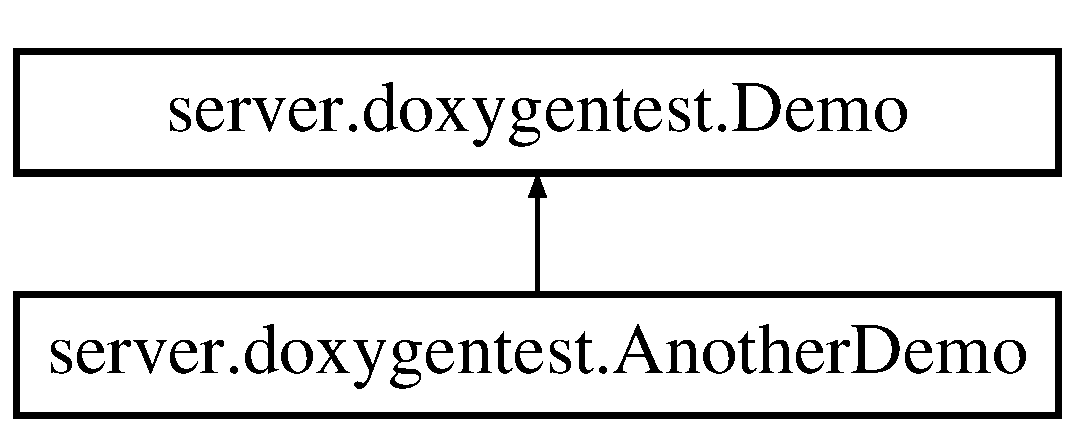
\includegraphics[height=2.000000cm]{classserver_1_1doxygentest_1_1_another_demo}
\end{center}
\end{figure}
\subsection*{Métodos públicos}
\begin{DoxyCompactItemize}
\item 
\hypertarget{classserver_1_1doxygentest_1_1_another_demo_a4e4707c541521e6e2f13020946624cb9}{def {\bfseries \-\_\-\-\_\-init\-\_\-\-\_\-}}\label{classserver_1_1doxygentest_1_1_another_demo_a4e4707c541521e6e2f13020946624cb9}

\end{DoxyCompactItemize}


\subsection{Descripción detallada}
\begin{DoxyVerb}\brief This class is derived from the demo class.\end{DoxyVerb}
 

La documentación para esta clase fue generada a partir del siguiente fichero\-:\begin{DoxyCompactItemize}
\item 
\hyperlink{doxygentest_8py}{doxygentest.\-py}\end{DoxyCompactItemize}

\hypertarget{classserver_1_1doxygentest_1_1_demo}{\section{Referencia de la Clase server.\-doxygentest.\-Demo}
\label{classserver_1_1doxygentest_1_1_demo}\index{server.\-doxygentest.\-Demo@{server.\-doxygentest.\-Demo}}
}
Diagrama de herencias de server.\-doxygentest.\-Demo\begin{figure}[H]
\begin{center}
\leavevmode
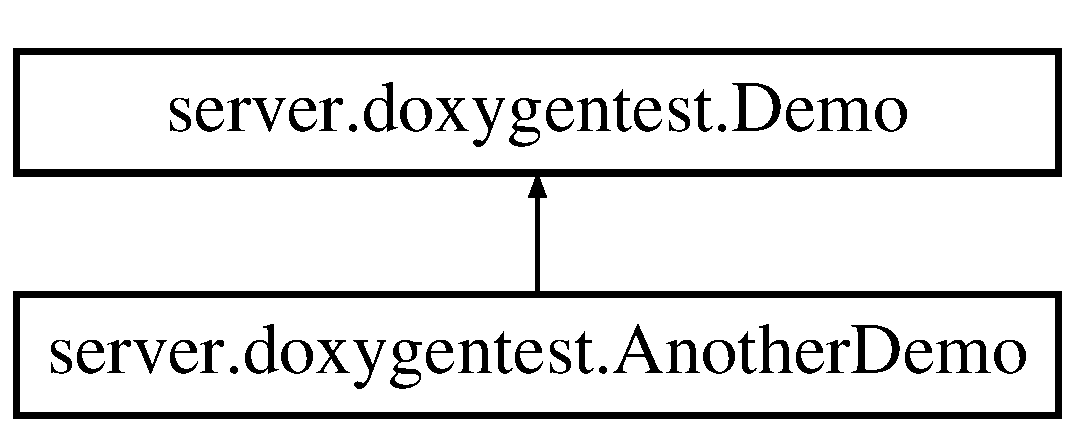
\includegraphics[height=2.000000cm]{classserver_1_1doxygentest_1_1_demo}
\end{center}
\end{figure}
\subsection*{Métodos públicos}
\begin{DoxyCompactItemize}
\item 
def \hyperlink{classserver_1_1doxygentest_1_1_demo_a5b398023230dee4667b322f95086aed7}{\-\_\-\-\_\-init\-\_\-\-\_\-}
\item 
def \hyperlink{classserver_1_1doxygentest_1_1_demo_a746219bba82e9e2d38b015448776f4b5}{foo}
\item 
def \hyperlink{classserver_1_1doxygentest_1_1_demo_afd773906bc6d63b962b58ea4b51d142a}{spam}
\begin{DoxyCompactList}\small\item\em protected\-: \end{DoxyCompactList}\end{DoxyCompactItemize}


\subsection{Descripción detallada}
\begin{DoxyVerb}\brief A demo class, it's really just for demonstration.

The detailed description of the class would appear right here.
However, as this class is utterly useless when talking about its
functionality it actually has no detailed description which is
sort of a pity, since a couple of lines of documentation would
make it look like a real documentation. But as this is just an
example of how the doxygen output might look like a one-liner has
to be enough. Insert your documentation here as appropriate. You
get the idea now, don't you? If not, I can't help it but I
certainly won't type in a lot of nonsense just to make it look \em
real.  No, definitely not.
\end{DoxyVerb}
 

\subsection{Documentación del constructor y destructor}
\hypertarget{classserver_1_1doxygentest_1_1_demo_a5b398023230dee4667b322f95086aed7}{\index{server\-::doxygentest\-::\-Demo@{server\-::doxygentest\-::\-Demo}!\-\_\-\-\_\-init\-\_\-\-\_\-@{\-\_\-\-\_\-init\-\_\-\-\_\-}}
\index{\-\_\-\-\_\-init\-\_\-\-\_\-@{\-\_\-\-\_\-init\-\_\-\-\_\-}!server::doxygentest::Demo@{server\-::doxygentest\-::\-Demo}}
\subsubsection[{\-\_\-\-\_\-init\-\_\-\-\_\-}]{\setlength{\rightskip}{0pt plus 5cm}def server.\-doxygentest.\-Demo.\-\_\-\-\_\-init\-\_\-\-\_\- (
\begin{DoxyParamCaption}
\item[{}]{self}
\end{DoxyParamCaption}
)}}\label{classserver_1_1doxygentest_1_1_demo_a5b398023230dee4667b322f95086aed7}
\begin{DoxyVerb}The constructor.\end{DoxyVerb}
 

\subsection{Documentación de las funciones miembro}
\hypertarget{classserver_1_1doxygentest_1_1_demo_a746219bba82e9e2d38b015448776f4b5}{\index{server\-::doxygentest\-::\-Demo@{server\-::doxygentest\-::\-Demo}!foo@{foo}}
\index{foo@{foo}!server::doxygentest::Demo@{server\-::doxygentest\-::\-Demo}}
\subsubsection[{foo}]{\setlength{\rightskip}{0pt plus 5cm}def server.\-doxygentest.\-Demo.\-foo (
\begin{DoxyParamCaption}
\item[{}]{self, }
\item[{}]{bar}
\end{DoxyParamCaption}
)}}\label{classserver_1_1doxygentest_1_1_demo_a746219bba82e9e2d38b015448776f4b5}
\begin{DoxyVerb}The infamous foo method.

There's no detailed description necessary for the \em foo()
function as everybody know what it does.

\param bar The \a bar argument is compulsory, never leave it out.
\return The \a bar input after processing by the \em foo() function.
\end{DoxyVerb}
 \hypertarget{classserver_1_1doxygentest_1_1_demo_afd773906bc6d63b962b58ea4b51d142a}{\index{server\-::doxygentest\-::\-Demo@{server\-::doxygentest\-::\-Demo}!spam@{spam}}
\index{spam@{spam}!server::doxygentest::Demo@{server\-::doxygentest\-::\-Demo}}
\subsubsection[{spam}]{\setlength{\rightskip}{0pt plus 5cm}def server.\-doxygentest.\-Demo.\-spam (
\begin{DoxyParamCaption}
\item[{}]{self, }
\item[{}]{amount}
\end{DoxyParamCaption}
)}}\label{classserver_1_1doxygentest_1_1_demo_afd773906bc6d63b962b58ea4b51d142a}


protected\-: 

\begin{DoxyVerb}Return an amount of spam.

\param amount (\c int) The amount of spam.
\return An amount of spam.
\end{DoxyVerb}
 

La documentación para esta clase fue generada a partir del siguiente fichero\-:\begin{DoxyCompactItemize}
\item 
\hyperlink{doxygentest_8py}{doxygentest.\-py}\end{DoxyCompactItemize}

\chapter{Documentación de archivos}
\hypertarget{doxygentest_8py}{\section{Referencia del Archivo doxygentest.\-py}
\label{doxygentest_8py}\index{doxygentest.\-py@{doxygentest.\-py}}
}


An example Python program.  


\subsection*{Clases}
\begin{DoxyCompactItemize}
\item 
class \hyperlink{classserver_1_1doxygentest_1_1_demo}{server.\-doxygentest.\-Demo}
\item 
class \hyperlink{classserver_1_1doxygentest_1_1_another_demo}{server.\-doxygentest.\-Another\-Demo}
\end{DoxyCompactItemize}


\subsection{Descripción detallada}
An example Python program. 
%--- End generated contents ---

% Index
\newpage
\phantomsection
\addcontentsline{toc}{chapter}{Índice}
\printindex

\end{document}
